\section{Estado del Arte y Antecedentes}

\subsection{2.1 Historia de Robótica en Órbitas}

Resulta revelador observar cómo los primeros intentos de robótica espacial orbitando la Tierra se remontan a finales del siglo pasado, cuando la comunidad internacional empezó a experimentar con manipuladores más allá de la simple teleoperación. Aunque los enfoques iniciales se limitaban a demostraciones básicas, sentaron las bases conceptuales para lo que hoy entendemos como operaciones de servicing y ensamblaje in-orbit.

Uno de los hitos más significativos surgió con el desarrollo de sistemas capaces de interactuar físicamente con otros vehículos en microgravedad. Estos esfuerzos pioneros revelaron desde temprano las complejidades únicas del entorno orbital: dinámica no lineal, ausencia de puntos fijos y perturbaciones constantes. En muchos casos estudiados, la latencia en comunicaciones y la necesidad de autonomía parcial se convirtieron en obstáculos persistentes que todavía hoy condicionan el diseño de sistemas.

\subsection{2.2 Misiones Representativas (OSAM-1, ETS-VII, etc.)}

Particularmente llamativo es el caso de ETS-VII, desarrollado por JAXA y lanzado en 1997. Este satélite demostró por primera vez operaciones autónomas de rendezvous y docking junto con un brazo robótico de dos metros capaz de realizar experimentos de manipulación. Sus logros fueron notables para la época, pero también expusieron limitaciones claras en precisión y capacidad de carga cuando se trata de estructuras de mayor escala.

Avanzando en el tiempo, proyectos más ambiciosos como OSAM-1 de NASA representaron un salto cualitativo al buscar integrar capacidades de refuel, ensamblaje y manufactura en una sola plataforma. Aunque la misión enfrentó desafíos técnicos, de costos y de programación que finalmente llevaron a su cancelación, sus objetivos y el trabajo de desarrollo asociado continúan influyendo en la hoja de ruta de tecnologías ISAM \cite{NASA_ISAM2025}. 

Otras plataformas, como Canadarm2 y Dextre en la Estación Espacial Internacional, han acumulado miles de horas de operación real, ofreciendo datos valiosos sobre manipulación prolongada. No obstante, cabe matizar que estos sistemas dependen fuertemente de control desde Tierra o tripulación, lo que reduce su aplicabilidad directa a misiones de exploración profunda donde la comunicación es intermitente o inexistente.

% Requiere únicamente \usepackage{booktabs} en el preámbulo

\begin{table}[!t]
\caption{Especificaciones Comparativas de Brazos Robóticos Espaciales Representativos}
\label{tab:especificaciones_brazos}
\centering
\footnotesize
\begin{tabular*}{\columnwidth}{@{\extracolsep{\fill}}l c c c c@{}}
\toprule
\textbf{Sistema} & \textbf{Longitud} & \shortstack{\textbf{Grados de}\\\textbf{Libertad}} & \shortstack{\textbf{Carga}\\\textbf{Máx. (kg)}} & \textbf{Año} \\
\midrule
ETS-VII Arm      & 2 m      & 6    & 10      & 1997 \\
Canadarm2        & 17 m     & 7    & 116,000 & 2001 \\
Dextre           & 3.5 m    & 7    & 600     & 2011 \\
\shortstack[l]{Prototipos\\OIRA} & Variable & 6--8 & 50--500 & 2023--2025 \\
\bottomrule
\end{tabular*}
\end{table}

\subsection{2.3 Revisiones Recientes y Tendencias}

Lejos de ser un asunto resuelto, la literatura reciente parece sugerir una maduración acelerada del campo. Revisiones exhaustivas clasifican las tecnologías de ensamblaje robótico in-orbit destacando el paso desde manipuladores teleoperados hacia sistemas con mayor grado de autonomía \cite{Wang2025_OASR}. 

Encuestas comprehensivas sobre manipuladores para on-orbit servicing subrayan el rol creciente de técnicas de estimación de estado y control basado en machine learning, aunque persisten brechas importantes en robustez frente a condiciones no nominales \cite{Alizadeh2024_Survey}. De forma paralela, análisis específicos de manipuladores autónomos para servicing y remoción de desechos espaciales enfatizan la necesidad de algoritmos que integren percepción, planificación y ejecución bajo incertidumbre \cite{Fallahiarezoodar2025_Manipulators}.

\begin{figure}[h]
\centering
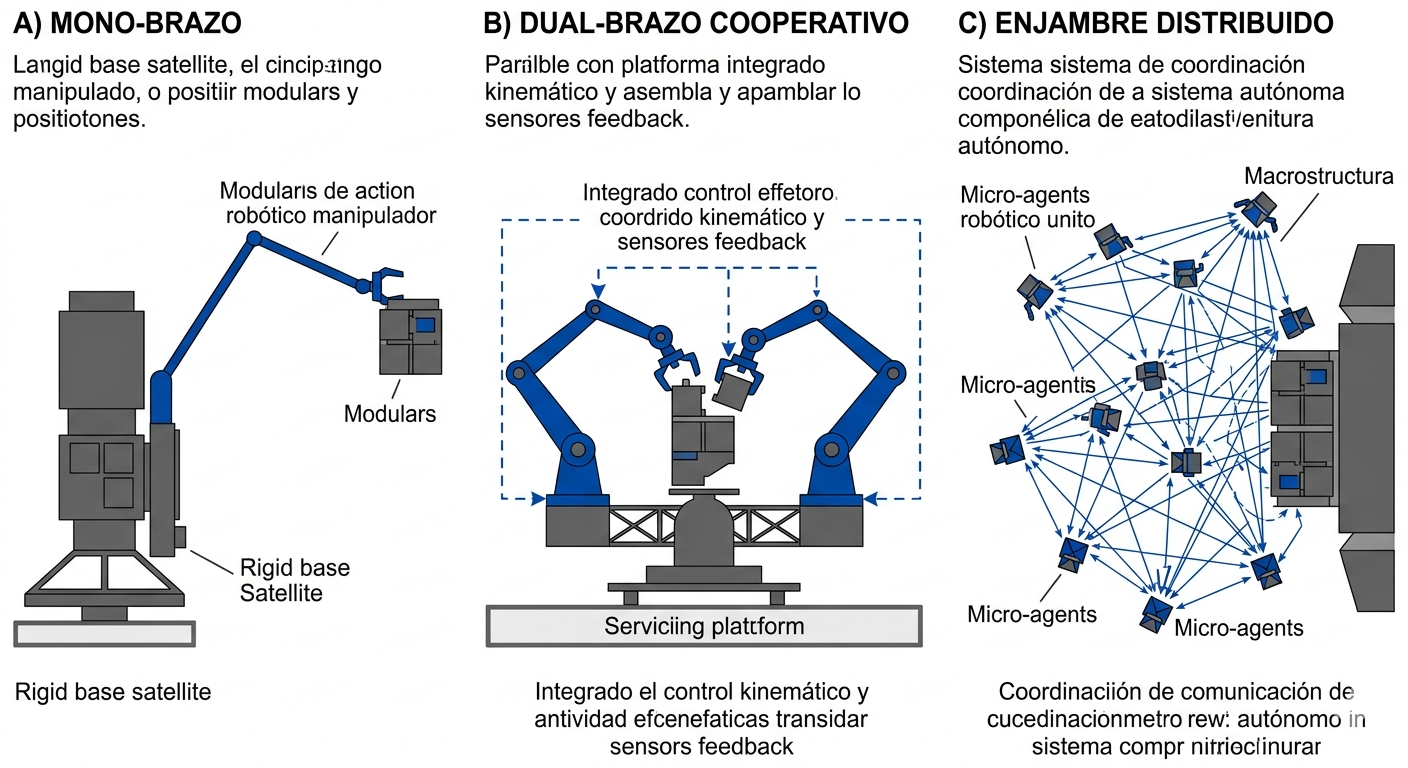
\includegraphics[width=\linewidth]{fig2.png}
\caption{Comparación esquemática de arquitecturas multi-robot para ensamblaje in-orbit: configuraciones mono-brazo, dual-brazo cooperativo y enjambre distribuido.}
\label{fig:arquitecturas_multi_robot}
\end{figure}

En conjunto, estas revisiones revelan una tendencia clara hacia la integración de gemelos digitales, planificación basada en IA y coordinación multi-robot. Aun así, la eficiencia energética y la reducción de riesgos en operaciones prolongadas siguen representando brechas críticas, especialmente cuando se proyectan hacia misiones de exploración profunda donde la intervención humana es inviable. El trabajo aquí presentado busca contribuir precisamente en estas áreas.